\subsection{Analyse des algorithmes Diviser-pour-Régner}

Le temps d'exécution $T(n)$ d'un algorithme diviser-pour-régner est décrit par une
\textbf{récurrence} de la forme :
\[
  T(n) =
  \begin{cases}
    \Theta(1)              & \text{si } n \le c, \\
    a\,T(n/b) + D(n) + C(n) & \text{sinon,}
  \end{cases}
\]
où $D(n)$ est le coût de la division et $C(n)$ celui de la combinaison. Pour le tri
fusion, cela donne $T(n) = 2T(n/2) + \Theta(n)$, soit $T(n) = \Theta(n\log n)$.

% ─────────────────────────────────────────────────────────────────────────────
\subsection{Résoudre les récurrences}

Il existe trois méthodes principales.

% ─────────────────────────────────────────────────────────────────────────────
\subsubsection{Méthode de substitution}

On \textbf{devine} la forme de la solution, puis on utilise l'induction mathématique
pour prouver les constantes.

\paragraph{Exemple : $T(n) = T(n/4 + 1) + T(3n/4 - 1) + \Theta(1)$.}
\emph{Montrons que $T(n) = O(n)$, i.e.\ $T(n) \le cn - d$ pour des constantes $c, d > 0$.}

\begin{proof}
Par hypothèse d'induction, les appels récursifs vérifient la borne. Avec $\Theta(1) \le k$ :
\begin{align*}
  T(n) &\le c\!\left(\tfrac{n}{4}+1\right) - d
          + c\!\left(\tfrac{3n}{4}-1\right) - d + k \\
       &= cn - 2d + k.
\end{align*}
Il suffit de choisir $d \ge k$ pour avoir $T(n) \le cn - d$. \qed
\end{proof}

% ─────────────────────────────────────────────────────────────────────────────
\subsubsection{Arbres de récursion}

On \textbf{visualise} le coût à chaque niveau de sous-problèmes. Utile pour générer
une conjecture à vérifier ensuite par substitution.

\begin{center}
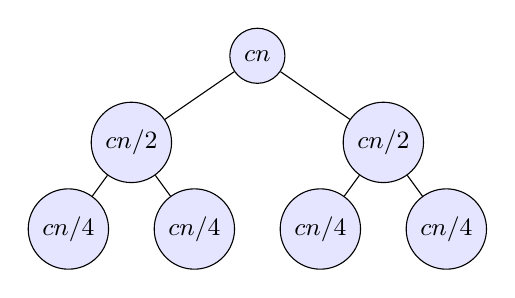
\begin{tikzpicture}[font=\small, level distance=1.1cm,
    level 1/.style={sibling distance=3.2cm},
    level 2/.style={sibling distance=1.6cm},
    every node/.style={circle, draw, fill=blue!10,
                       inner sep=3pt, minimum size=0.7cm}]
  \node {$cn$}
    child { node {$cn/2$}
      child { node {$cn/4$} }
      child { node {$cn/4$} }
    }
    child { node {$cn/2$}
      child { node {$cn/4$} }
      child { node {$cn/4$} }
    };
\end{tikzpicture}
\quad
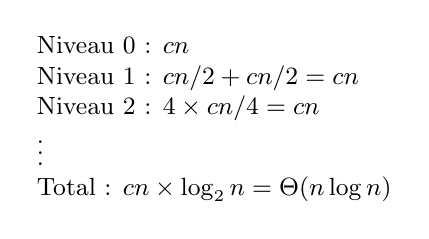
\begin{tikzpicture}[font=\small, baseline=0pt]
  \node[align=left]{
    Niveau 0 : $cn$\\
    Niveau 1 : $cn/2 + cn/2 = cn$\\
    Niveau 2 : $4 \times cn/4 = cn$\\
    $\vdots$\\
    Total : $cn \times \log_2 n = \Theta(n\log n)$
  };
\end{tikzpicture}
\end{center}

% ─────────────────────────────────────────────────────────────────────────────
\subsubsection{Master Theorem (Théorème Maître)}

Recette pour les récurrences de la forme $T(n) = aT(n/b) + f(n)$
(avec $a \ge 1$, $b > 1$). On compare $f(n)$ et $n^{\log_b a}$ :

\begin{center}
\renewcommand{\arraystretch}{1.5}
\begin{tabular}{clll}
\toprule
\textbf{Cas} & \textbf{Condition sur $f(n)$} & \textbf{Résultat} & \textbf{Intuition} \\
\midrule
1 & $f(n) = O\!\left(n^{\log_b a - \varepsilon}\right)$, $\varepsilon>0$
  & $T(n) = \Theta\!\left(n^{\log_b a}\right)$
  & Les feuilles dominent \\
2 & $f(n) = \Theta\!\left(n^{\log_b a}\right)$
  & $T(n) = \Theta\!\left(n^{\log_b a}\log n\right)$
  & Coût équiparti \\
3 & $f(n) = \Omega\!\left(n^{\log_b a + \varepsilon}\right)$, $\varepsilon>0$
  & $T(n) = \Theta(f(n))$
  & La racine domine \\
\bottomrule
\end{tabular}
\end{center}

\textbf{Exemples d'application :}
\begin{itemize}
  \item Merge Sort : $T(n) = 2T(n/2) + \Theta(n)$.
        Ici $a=2$, $b=2$, $n^{\log_2 2} = n$. Cas~2 $\Rightarrow T(n)=\Theta(n\log n)$.
  \item Recherche binaire : $T(n) = T(n/2) + \Theta(1)$.
        Ici $n^{\log_2 1} = 1$. Cas~2 $\Rightarrow T(n)=\Theta(\log n)$.
  \item Strassen : $T(n) = 7T(n/2) + \Theta(n^2)$.
        $n^{\log_2 7} \approx n^{2.81} \succ n^2$. Cas~1 $\Rightarrow T(n)=\Theta(n^{\log_2 7})$.
\end{itemize}

% ─────────────────────────────────────────────────────────────────────────────
\subsection{Problème du sous-tableau maximum}

\textbf{Entrée :} un tableau $A[low \ldots high]$ de $n$ entiers (certains négatifs).\\
\textbf{Sortie :} les indices $i, j$ et la somme $\sum_{k=i}^{j} A[k]$ maximale.

\subsubsection{Approche diviser-pour-régner}

On divise $A$ en deux moitiés $A[low \ldots mid]$ et $A[mid{+}1 \ldots high]$.
Le sous-tableau maximal est soit :

\begin{enumerate}
  \item Entièrement dans la moitié \textbf{gauche},
  \item Entièrement dans la moitié \textbf{droite},
  \item \textbf{Traversant le milieu} (une partie à gauche de $mid$, une à droite).
\end{enumerate}

\begin{center}
\begin{tikzpicture}[font=\small]
  \draw[fill=blue!8] (0,0) rectangle (4,0.7);
  \draw[fill=orange!20] (4,0) rectangle (8,0.7);
  \draw[dashed, thick] (4,-0.2) -- (4,0.9);
  \node at (2, 0.35) {gauche};
  \node at (6, 0.35) {droite};
  \node[below] at (4, -0.25) {$mid$};
  % Crossing subarray highlight
  \draw[keyred, very thick] (2.5, 0) rectangle (5.8, 0.7);
  \node[keyred, above] at (4.15, 0.75) {\small traversant};
\end{tikzpicture}
\end{center}

La fonction \textsc{Find-Max-Crossing-Subarray} scanne depuis $mid$ vers la gauche puis
vers la droite en $\Theta(n)$. La récurrence globale est :
\[
  T(n) = 2T(n/2) + \Theta(n) \;\Rightarrow\; \boxed{T(n) = \Theta(n \log n)}
\]